\section{kNN分类器实现}
\subsection{kNN原理介绍}
\subsubsection{什么是kNN}
k最近邻(kNN,k-NearestNeighbor)分类算法是数据挖掘分类技术中最简单的方法之一。所谓K最近邻,就是
k个最近的邻居的意思,说的是每个样本都可以用它最接近的k个邻居来代表。

kNN算法的核心思想是如果一个样本在特征空间中的k个最相邻的样本中的大多数属于某一个类别,则该样本也
属于这个类别,并具有这个类别上样本的特性。该方法在确定分类决策上只依据最邻近的一个或者几个样本的
类别来决定待分样本所属的类别。 kNN方法在类别决策时,只与极少量的相邻样本有关。由于kNN方法主要靠
周围有限的邻近的样本,而不是靠判别类域的方法来确定所属类别的,因此对于类域的交叉或重叠较多的待分样
本集来说,kNN方法较其他方法更为适合。

下面通过一个简单的例子说明一下:如下图,绿色圆要被决定赋予哪个类,是红色三角形还是蓝色四方形?
如果K=3,由于红色三角形所占比例为2/3,绿色圆将被赋予红色三角形那个类,如果K=5,由于蓝色四方形
比例为3/5,因此绿色圆被赋予蓝色四方形类。由此也说明了kNN算法的结果很大程度取决于K的选择。

\begin{figure}[thbp!]
  \centering
  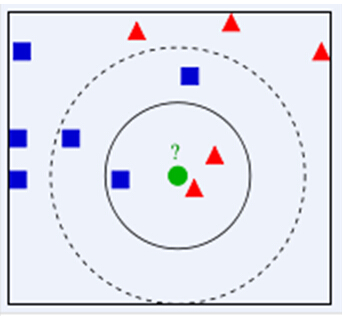
\includegraphics[width=0.4\linewidth]{figure/KNN/KNNIntro.png}
  \caption{kNN原理介绍图}
  \label{fig:KNNIntro}
\end{figure}

在kNN中,通过计算对象间距离来作为各个对象之间的非相似性指标,避免了对象之间的匹配问题,
在这里距离一般使用欧氏距离$d(x,y)=\sqrt{\sum_{k=1}^N (x_k-y_k)^2}$或曼哈顿距离
$d(x,y)=\sum_{k=1}^N \left|x_k-y_k\right|$。
同时,KNN通过依据k个对象中占优的类别进行决策,而不是单一的对象类别决策。这两点就是KNN算法的优势。

\subsubsection{kNN算法流程}
接下来对KNN算法的思想总结一下:就是在训练集中数据和标签已知的情况下,输入测试数据,将测试数据的特
征与训练集中对应的特征进行相互比较,找到训练集中与之最为相似的前K个数据,则该测试数据对应的类别
就是K个数据中出现次数最多的那个分类,其算法的描述为:
% \begin{algorithm}
%   \caption{kNN算法}
%   \label{alg:kNN}
%   \begin{algorithmic}
%     \STATE {set $r(t)=x(t)$} 
%     \REPEAT 
%     \STATE set $h(t)=r(t)$ 
%     \REPEAT
%     \STATE set $h(t)=r(t)$ 
%     \UNTIL{B} 
%     \UNTIL{B}
%   \end{algorithmic}
% \end{algorithm}
\begin{algorithm}
  \caption{kNN算法}
  \label{alg:kNN}
  \begin{algorithmic}
    \STATE {1.计算测试数据与各个训练数据之间的距离} 
    \STATE {2.按照距离的递增关系进行排序} 
    \STATE {3.选取距离最小的k个点} 
    \STATE {4.确定前k个点所在类别的出现频率} 
    \STATE {5.返回前k个点中出现频率最高的类别作为测试数据的预测分类}     
  \end{algorithmic}
\end{algorithm}

\subsection{数据预处理}
从\ref{Ch:Mnist}我们已经从Mnist数据集读取了我们训练分类器所需要的图片和标签数据,
然而得到的图片是28*28的数组,为了便于后续计算,我们需要将二维数组转为一维数组。
\begin{python}
  # 训练集图片
  train_input=train_images.reshape((train_images.shape[0],train_images.shape[1]*train_images.shape[2]),order='F')
  #测试集图片
  test_input=test_images.reshape((test_images.shape[0],test_images.shape[1]*test_images.shape[2]),order='F')
\end{python}

\subsection{kNN实现}
\subsubsection{计算距离矩阵}
对于后续选合适的k值时,不用再重新计算距离矩阵。
\begin{python}
  def ComputerDistanceMat(testdata,traindata,testsize):
    #将序列转换成矩阵
    testdata=np.mat(testdata)   
    traindata=np.mat(traindata)
    #获取traindata的第一维大小
    trainsize=traindata.shape[0]
    distancesort_mat=np.mat(np.zeros(shape=(testsize,trainsize)))
    for i in range(testsize):
        X=testdata[i,:]
        #计算L1
        distance=np.sum(np.array(np.tile(X,(trainsize,1))-traindata)**2,1)
        distancesort = distance.argsort()
        distancesort_mat[i]=distancesort
    return distancesort_mat
\end{python}

\subsubsection{kNN分类器}
\begin{python}
  def KNN(distancesort_mat,trainlabel,testsize,k):
    ret_pred=[]
    trainlabel=np.mat(trainlabel)
    for i in range(distancesort_mat.shape[0]):
        countdict = dict()
        for j in range(k):
            Xlabel= trainlabel[0,int(distancesort_mat[i,j])]#distancesort存储的是训练数据集的索引
            countdict[Xlabel] = countdict.get(Xlabel,0) + 1
        countlist = sorted(countdict.items(),key=lambda x:x[1],reverse = True)
        ret_pred.append(countlist[0][0])
    return ret_pred
\end{python}
\subsubsection{计算召回率}
\begin{python}
  def compute(ret_pred,testlabel,testsize,k):
    error=0
    for i in range(0,testsize):
        if(ret_pred[i]!=testlabel[i]):
            error+=1
    return 1-error/testsize
\end{python}
\subsubsection{选取合适的k}
我们知道不同的k影响最终的分类准确率,因此我们需要通过实验选取合适的k。
\begin{python}
  accuracy=np.zeros(shape=(50,1))
  print("start")
  for k in range(1,50):
    ret_pred=KNN(distancesort_mat,train_labels,testsize,k)
    ac_temp=compute(ret_pred,test_labels,testsize,k)
    accuracy[k]=ac_temp
    print("k:",k,"accuracy:",ac_temp)
  print("end")
\end{python}
\subsection{kNN分类器训练结果}
\begin{figure}[htbp]
  \centering
  \begin{minipage}[t]{0.48\textwidth}
    \centering
    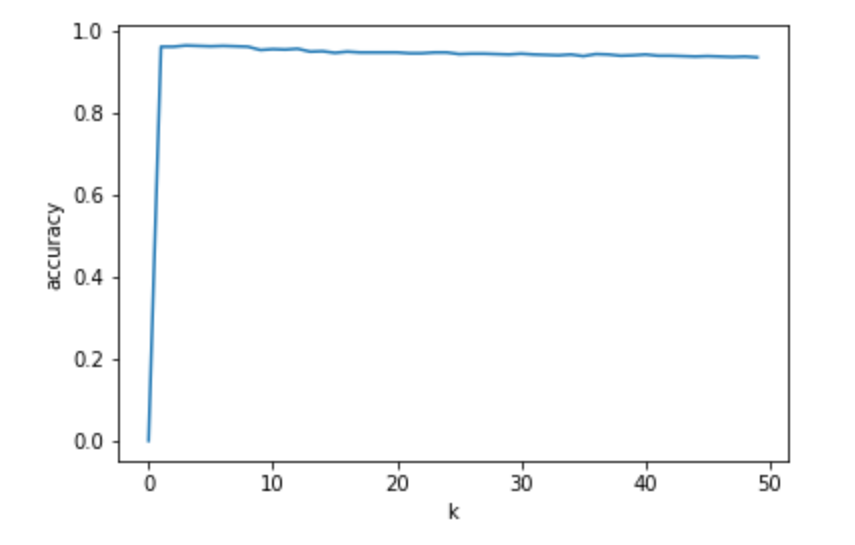
\includegraphics[width=7.5cm]{figure/KNN/kfig.png}
    \caption{不同k对应的准确率}
    \label{fig:ch1KFig}
  \end{minipage}
  \begin{minipage}[t]{0.48\textwidth}
    \centering
    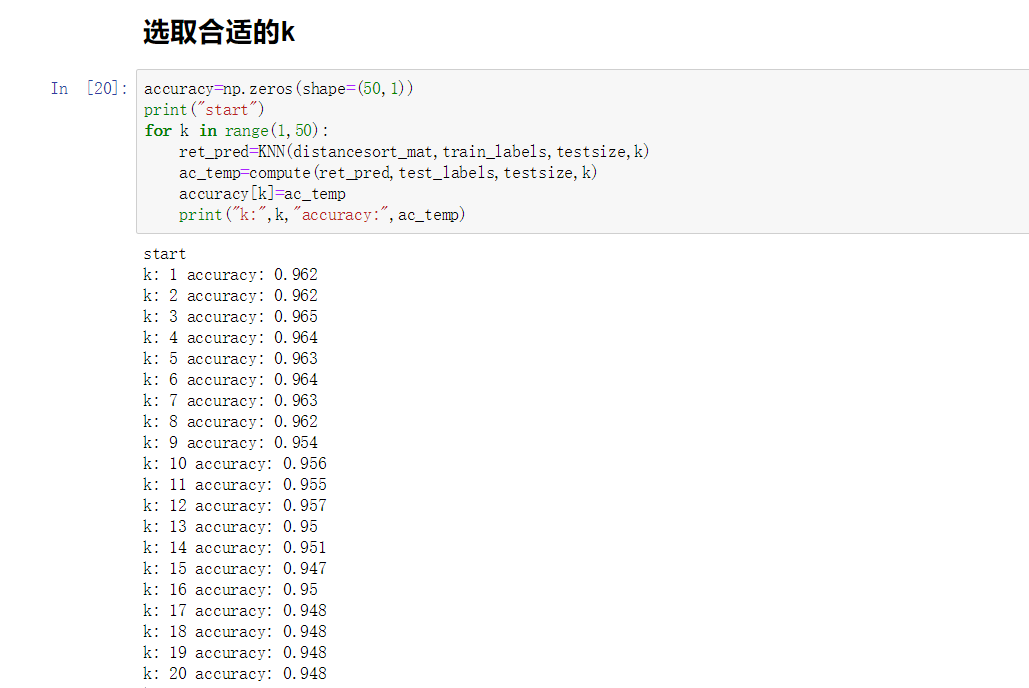
\includegraphics[width=7.5cm]{figure/KNN/kret.png}
    \caption{k对应准确率}
    \label{fig:ch1KRet}
  \end{minipage}
\end{figure}
右图\ref{fig:ch1KRet}可以看出,当我们选取k为3时可以得到较好的分类准确率,并且运算量相对较少。

